% Figure 3: one printed joint classification, and four readings of it.
% Numbers: results/figure_one_table.json (Guerra et al. 2026, N = 20,306).
% House vocabulary: HOUSE_STYLE/docs/viz.md. Compile: pdflatex fig_four_readings.tex
\documentclass[tikz,border=6pt]{standalone}
\usepackage{amsmath,amssymb}
\usetikzlibrary{arrows.meta,positioning,calc}

\definecolor{boxblue}{HTML}{DBEAFE}  \definecolor{bordblue}{HTML}{3B82F6}
\definecolor{anncolor}{HTML}{6B7280} \definecolor{ink}{HTML}{1B2A41}

\begin{document}
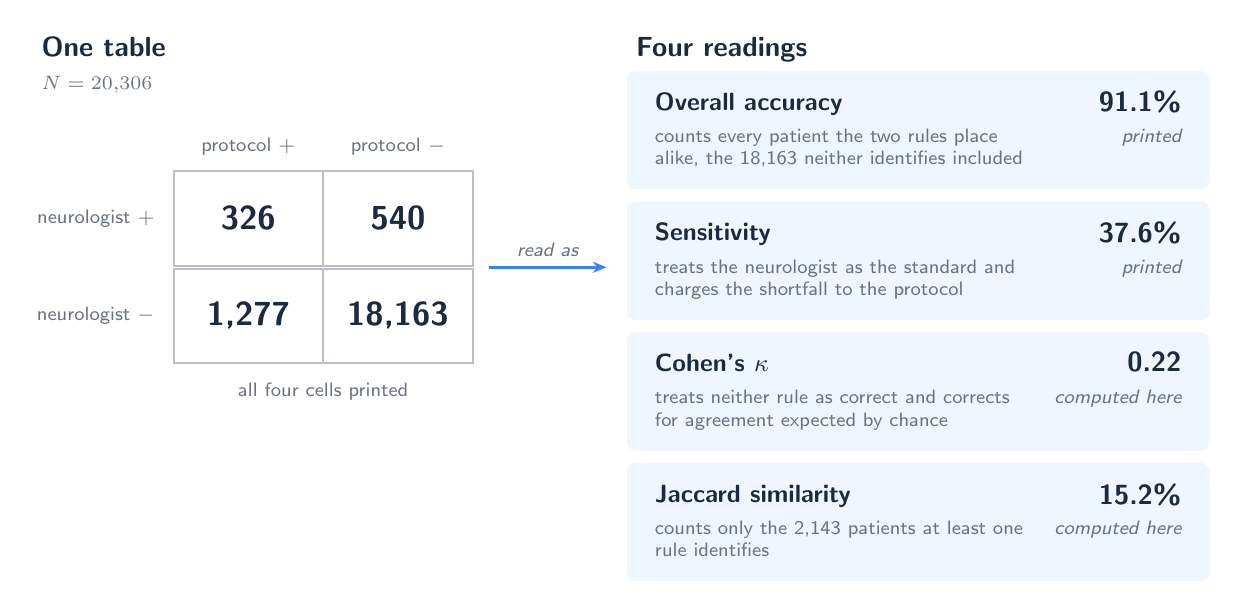
\begin{tikzpicture}[
    font=\sffamily,
    cell/.style={rectangle, minimum width=1.9cm, minimum height=1.2cm, text centered,
                 font=\sffamily\bfseries\large, draw=anncolor!45, line width=0.7pt,
                 fill=white, text=ink},
    hdr/.style={font=\sffamily\scriptsize, color=anncolor},
    title/.style={font=\sffamily\bfseries, color=ink},
    card/.style={rectangle, rounded corners=3pt, fill=boxblue!45, minimum width=7.4cm,
                 minimum height=1.5cm, anchor=north west},
    cardname/.style={font=\sffamily\bfseries\small, color=ink, anchor=north west},
    cardval/.style={font=\sffamily\bfseries, color=ink, anchor=north east},
    cardtag/.style={font=\sffamily\scriptsize\itshape, color=anncolor, anchor=north east},
    cardnote/.style={font=\sffamily\scriptsize, color=anncolor, anchor=north west,
                     align=left, text width=4.7cm},
    onarrow/.style={font=\sffamily\scriptsize\itshape, color=anncolor},
    arr/.style={-{Stealth[length=5pt,width=4pt]}, line width=1.1pt, color=bordblue},
]

%% ---- what the registry printed ---------------------------------------------
\node[title, anchor=north west] at (-1.75,3.05) {One table};
\node[hdr,   anchor=north west] at (-1.75,2.55) {$N = 20{,}306$};

\node[cell] (c11) at (1.0,0.62)  {326};
\node[cell] (c10) at (2.9,0.62)  {540};
\node[cell] (c01) at (1.0,-0.62) {1{,}277};
\node[cell] (c00) at (2.9,-0.62) {18{,}163};
\node[hdr, above=2pt of c11] {protocol $+$};   \node[hdr, above=2pt of c10] {protocol $-$};
\node[hdr, left=3pt of c11] {neurologist $+$}; \node[hdr, left=3pt of c01] {neurologist $-$};
\node[hdr, anchor=north] at (1.95,-1.35) {all four cells printed};

\draw[arr] (4.05,0) -- node[onarrow, above] {read as} (5.55,0);

%% ---- four readings computed from it ----------------------------------------
\node[title, anchor=north west] at (5.8,3.05) {Four readings};

\node[card] (r1) at (5.8,2.5)   {};
\node[card] (r2) at (5.8,0.84)  {};
\node[card] (r3) at (5.8,-0.82) {};
\node[card] (r4) at (5.8,-2.48) {};

\node[cardname] at ($ (r1.north west) + (0.24,-0.16) $) {Overall accuracy};
\node[cardval]  at ($ (r1.north east) + (-0.24,-0.14) $) {91.1\%};
\node[cardtag]  at ($ (r1.north east) + (-0.24,-0.62) $) {printed};
\node[cardnote] at ($ (r1.north west) + (0.24,-0.62) $)
    {counts every patient the two rules place alike, the 18,163 neither identifies included};

\node[cardname] at ($ (r2.north west) + (0.24,-0.16) $) {Sensitivity};
\node[cardval]  at ($ (r2.north east) + (-0.24,-0.14) $) {37.6\%};
\node[cardtag]  at ($ (r2.north east) + (-0.24,-0.62) $) {printed};
\node[cardnote] at ($ (r2.north west) + (0.24,-0.62) $)
    {treats the neurologist as the standard and charges the shortfall to the protocol};

\node[cardname] at ($ (r3.north west) + (0.24,-0.16) $) {Cohen's $\kappa$};
\node[cardval]  at ($ (r3.north east) + (-0.24,-0.14) $) {0.22};
\node[cardtag]  at ($ (r3.north east) + (-0.24,-0.62) $) {computed here};
\node[cardnote] at ($ (r3.north west) + (0.24,-0.62) $)
    {treats neither rule as correct and corrects for agreement expected by chance};

\node[cardname] at ($ (r4.north west) + (0.24,-0.16) $) {Jaccard similarity};
\node[cardval]  at ($ (r4.north east) + (-0.24,-0.14) $) {15.2\%};
\node[cardtag]  at ($ (r4.north east) + (-0.24,-0.62) $) {computed here};
\node[cardnote] at ($ (r4.north west) + (0.24,-0.62) $)
    {counts only the 2,143 patients at least one rule identifies};

\end{tikzpicture}
\end{document}
